\documentclass{beamer}
\mode<presentation>{\usetheme{Copenhagen}}

\usepackage{etoolbox}
\makeatletter
\patchcmd{\insertverticalnavigation}%
{\ifx\beamer@nav@css\beamer@hidetext{\usebeamertemplate{section in sidebar}}\else{\usebeamertemplate{section in sidebar shaded}}\fi}%
{{\usebeamertemplate{section in sidebar}}}{}{}
\makeatother
\title{Machine Learning in Astronomy}
\author{Reza Monadi}
\institute{UC Riverside}
\date{May 14, 2020}
\begin{document}
	
	\frame{\titlepage}
	
	\begin{frame}
	\centering
	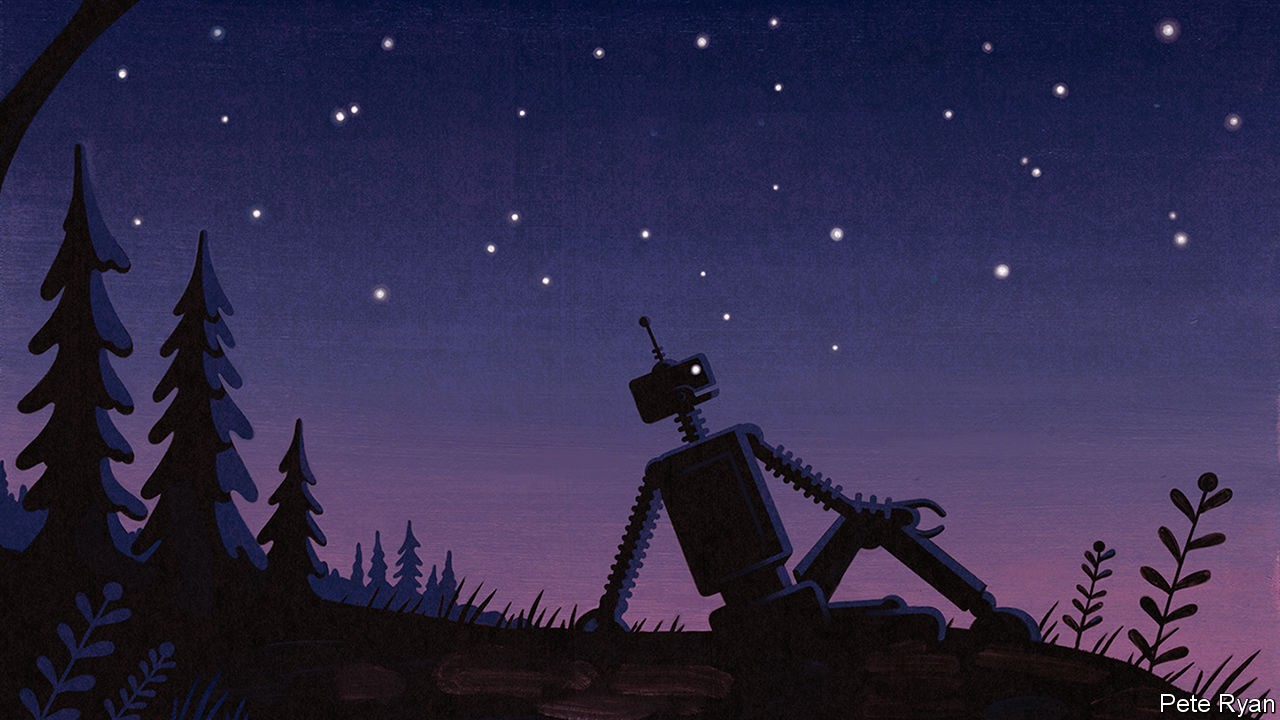
\includegraphics[height=6cm, angle=0,origin=c]{ml2.jpeg}
	
\end{frame}

	
\section{Questions to be addresses}
\frame{
	\begin{itemize}
		\uncover<1->{\item Is \textbf{ML} the same as \textbf{Statistics} or \textbf{Computer Science}?}
%		\uncover<2->{\item How big is \textbf{BIG DATA}?}
		\uncover<2->{\item How \textbf{ML} is tied to \textbf{BIG DATA}?}
		\uncover<3->{\item How to implement \textbf{ML} in astronomy? }
		\uncover<4->{\item How \textbf{ML} helps \textbf{SKA}?}
		\uncover<5->{\item What are the pitfalls of \textbf{ML}?}
	\end{itemize}
	}

\section{Machine learning overview}\frame{text}
\subsection{a}\frame{}
\subsection{b}\frame{}
\section{Big Data in Astronomy}\frame{
\centering
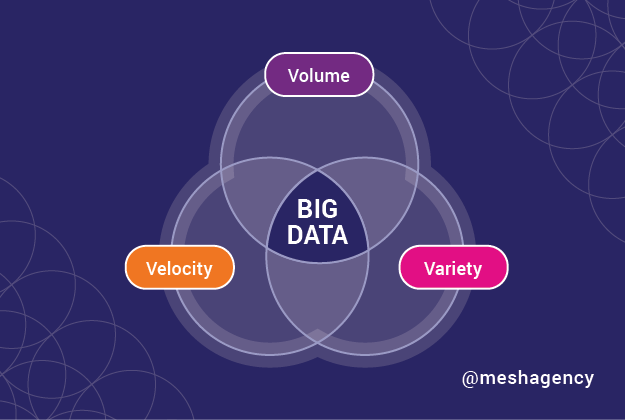
\includegraphics[height=6cm, angle=0,origin=c]{vvv.png}
}
\subsection{a}\frame{}
\subsection{b}\frame{}

\section{ML methods for astronomy}\frame{text}
\subsection{a}\frame{}
\subsection{b}\frame{}

\section{SKA: a practical example}\frame{text}
\subsection{a}\frame{}
\subsection{b}\frame{}
\section{ML limitations}\frame{text}
\subsection{a}\frame{}
\subsection{b}\frame{}
\end{document}